\section{RoboDK}

RoboDK is a development platform for industrial robot offline programming and simulation.

\subsection{RoboDK history}

RoboDK (the company) was founded by Albert Nubiola and Lauren Ierullo in January 2015 as a spin-off company from the \href{https://en.etsmtl.ca/unites-de-recherche/coro/accueil?lang=en-CA}{CoRo laboratory}   at ETS University in Montreal, Canada. RoboDK is a commercial version of RoKiSim, a multi-platform educational software tool for 3D simulation of serial six-axis robots.

\subsection{RoboDK features}

RoboDK is a CAM (Computer-aided manufacturing) simulator for industrial robots and robot programming. Mobile robots are not supported. 

RoboDK supports offline programming and has an extensive robot library supporting many robot controllers, including:

\begin{itemize}
    \item ABB RAPID (mod/prg)
    \item Fanuc LS (LS/TP)
    \item KUKA KRC/IIWA (SRC/java)
    \item Motoman Inform (JBI)
    \item Universal Robots (URP/script)
\end{itemize}

RoboDK offers a free (limited), educational or professional version. 
The software is available for Windows, Mac OS, Ubuntu Linux or Android. It supports either 32 or 64-bit versions of the abovementioned operating systems. The logo of RoboDK is shown in Figure No.\ref{fig:robodklogo}.

\begin{figure}[htp]
    \centering
    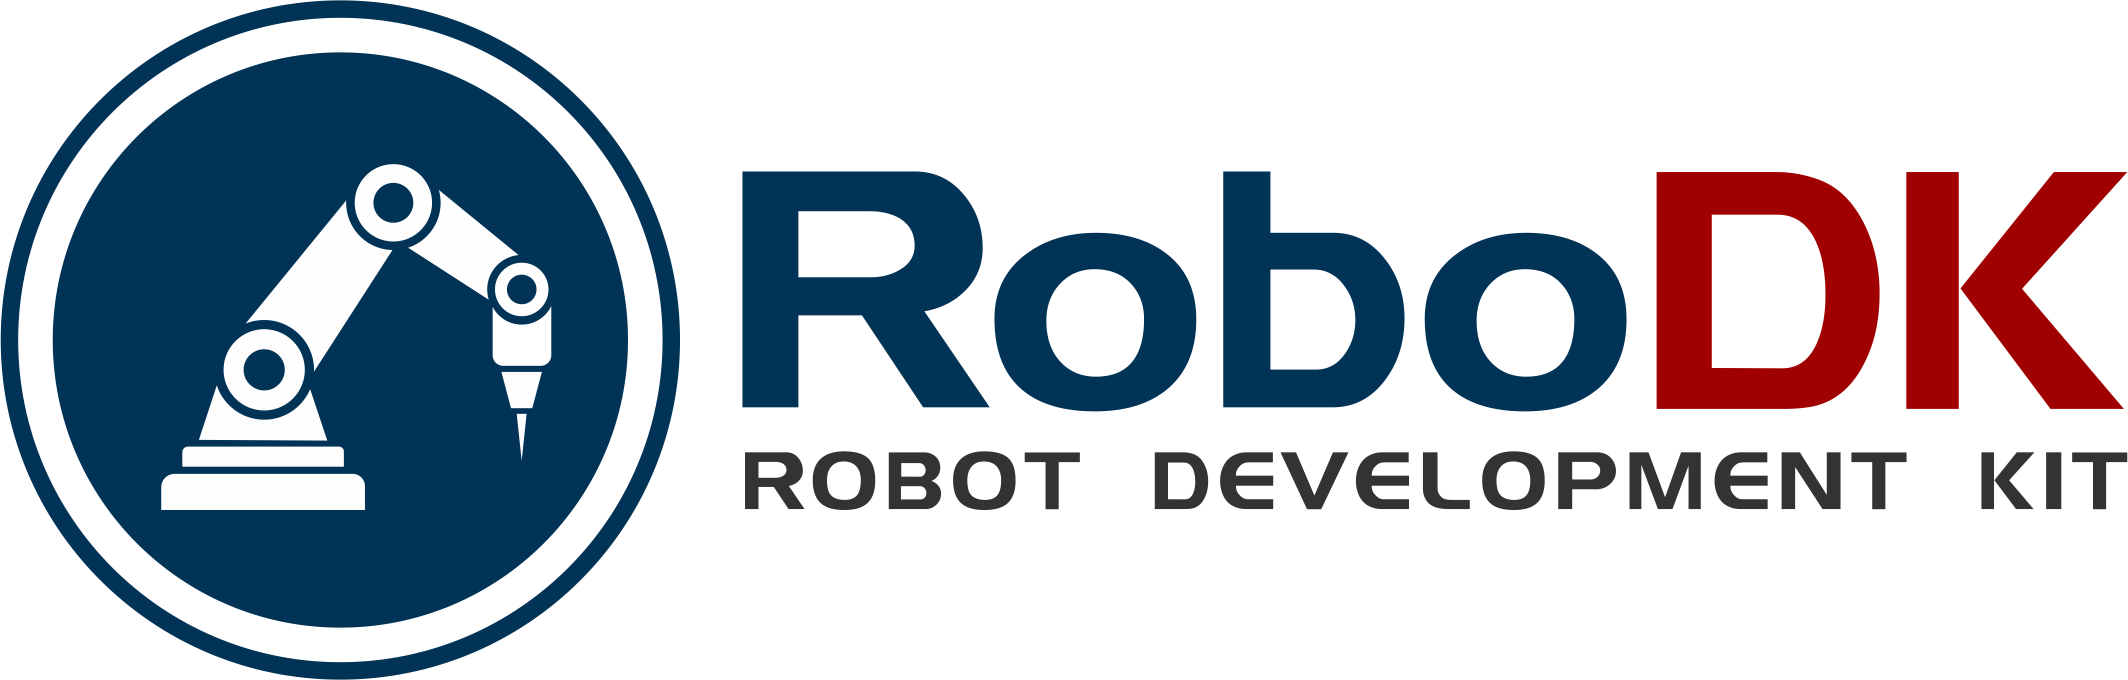
\includegraphics[width=0.9\linewidth]{img/robodk_logo.png}
    \caption{RoboDK logo.}
    \label{fig:robodklogo}
\end{figure}

\subsection{RoboDK interface}

The interface of RoboDK consists of the main menu, the toolbar, the station tree, the status bar and the 3D view. A picture of the RoboDK interface is shown in Figure No \ref{fig:robodkinterface}. An extensive API for RoboDK is available \href{https://robodk.com/doc/en/Basic-Guide.html#Start}{online}.


\begin{figure}[h]
    \centering
    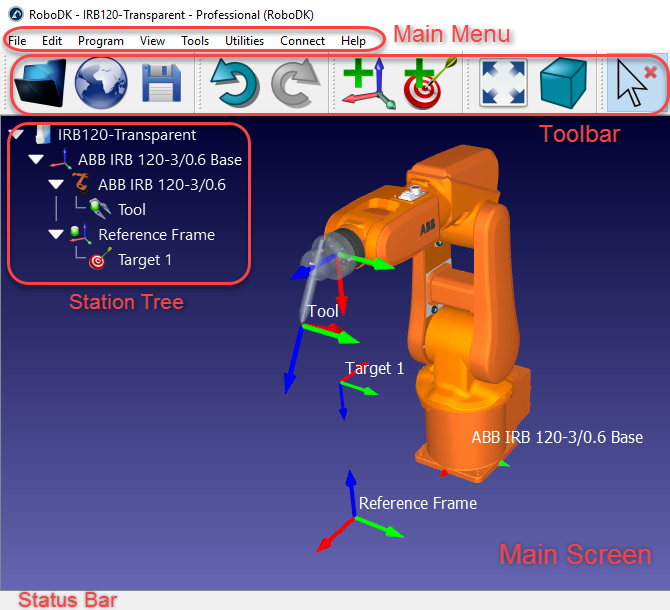
\includegraphics[width=0.9\linewidth]{img/robodk_interface.png}
    \caption{RoboDK interface.}
    \label{fig:robodkinterface}
\end{figure}

\subsection{RoboDK API}
